
\documentclass[../main.tex]{subfiles}




\begin{document}

\noindent We used \texttt{R} for this study and you may find the related codes as well as some analysis in this section.

\subsection{Data Pre-Processing}
\noindent The first part of our study was data pre-processing which includes: 1) variable selection 2) outlier detection 3) variable transformation. As mentioned we used Lasso for variable selection. We can get a rough idea of important variables by looking at the correlation between all predictors:






\vspace{1cm}
\subsubsection{Variable Selection}
\begin{Shaded}
\begin{Highlighting}[]
\CommentTok{## Read Data}
\KeywordTok{set.seed}\NormalTok{(}\DecValTok{123}\NormalTok{)}
\NormalTok{Red_wine =}\StringTok{ }\KeywordTok{read.csv}\NormalTok{(}\StringTok{"winequality-red.csv"}\NormalTok{)}
\NormalTok{Missed.data =}\StringTok{ }\KeywordTok{sum}\NormalTok{(}\KeywordTok{is.na}\NormalTok{(Red_wine))}
\NormalTok{var.name=}\KeywordTok{colnames}\NormalTok{(Red_wine)}
\end{Highlighting}
\end{Shaded}

\begin{Shaded}
\begin{Highlighting}[]
\NormalTok{split =}\StringTok{ }\NormalTok{Red_wine}\OperatorTok{\$}\NormalTok{quality}
\KeywordTok{plot}\NormalTok{(Red_wine[,}\OperatorTok{-}\KeywordTok{c}\NormalTok{(}\DecValTok{12}\NormalTok{)], }\DataTypeTok{pch =} \DecValTok{19}\NormalTok{, }\DataTypeTok{col =}\NormalTok{ split, }\DataTypeTok{cex =} \FloatTok{0.4}\NormalTok{)}
\KeywordTok{corrplot}\NormalTok{(}\KeywordTok{cor}\NormalTok{(Red_wine[,}\OperatorTok{-}\KeywordTok{c}\NormalTok{(}\DecValTok{12}\NormalTok{)]),}\DataTypeTok{method =} \StringTok{"circle"}\NormalTok{)}
\end{Highlighting}
\end{Shaded}

\begin{figure}[H]
\begin{minipage}[]{.4\textwidth}
    \centering
    \includegraphics[scale=0.5]{Correlation.PNG}
    \label{fig:Cor1}
\end{minipage}
\hspace{0.5cm}
\begin{minipage}[]{.6\textwidth}
    \centering
    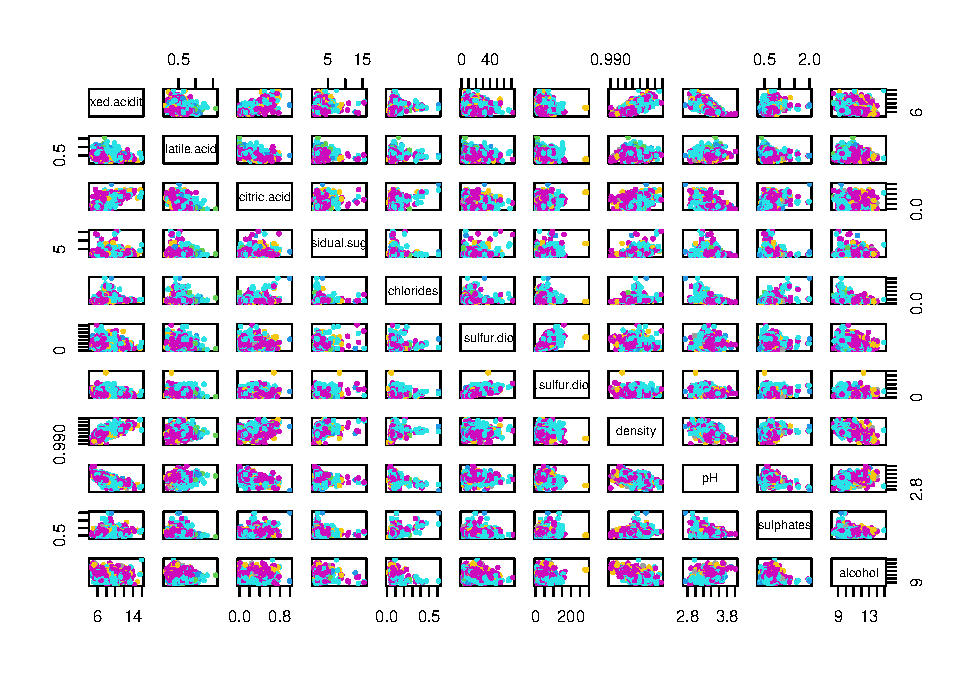
\includegraphics[scale=0.6]{AppendixFiles/Correlation-1.pdf}
    \label{fig:Cor2}
\end{minipage}
\end{figure}





\noindent As the left plot shows, \texttt{fixed.acidity}, \texttt{citric.acid}, \texttt{density} and \texttt{pH} are highly correlated. Ther is also high correlation among \texttt{free.sulfur.dioxide} and \texttt{total.sulfur.dioxide}. So we may remove some of them to avoid co-linearity. Pair-plot of the predictors is shown on the right hand side. In this plot, observations are colored according to their quality level. The plot indicates that no single predictor is able to classify wines based on their quality. Now we may use lasso to select useful variables in a more systematic way.

\vspace{0.5cm}
\begin{Shaded}
\begin{Highlighting}[]
\CommentTok{# Splitting the Data}
\NormalTok{train=}\KeywordTok{sample}\NormalTok{(}\DecValTok{1}\OperatorTok{:}\KeywordTok{nrow}\NormalTok{(Red_wine), }\KeywordTok{floor}\NormalTok{(}\KeywordTok{nrow}\NormalTok{(Red_wine) }\OperatorTok{*}\StringTok{ }\FloatTok{0.8}\NormalTok{))}
\NormalTok{test=(}\DecValTok{1}\OperatorTok{:}\KeywordTok{nrow}\NormalTok{(Red_wine))[}\OperatorTok{-}\NormalTok{train]}
\NormalTok{Red_wine.train =}\StringTok{ }\NormalTok{Red_wine[train,]}
\NormalTok{Red_wine.test =}\StringTok{ }\NormalTok{Red_wine[test,]}
\end{Highlighting}
\end{Shaded}

\begin{Shaded}
\begin{Highlighting}[]
\KeywordTok{library}\NormalTok{(glmnet)}
\NormalTok{data.matrix =}\StringTok{ }\KeywordTok{model.matrix}\NormalTok{(quality }\OperatorTok{~}\StringTok{ }\NormalTok{.,}
\NormalTok{                           Red_wine.train)}
\NormalTok{xtrain =}\StringTok{ }\NormalTok{data.matrix[,}\OperatorTok{-}\DecValTok{1}\NormalTok{]}
\NormalTok{ytrain =}\StringTok{ }\NormalTok{Red_wine.train}\OperatorTok{\$}\NormalTok{quality}
\KeywordTok{set.seed}\NormalTok{(}\DecValTok{123}\NormalTok{)}
\NormalTok{cv.lasso <-}\StringTok{ }\KeywordTok{cv.glmnet}\NormalTok{(xtrain, ytrain, }\DataTypeTok{alpha =} \DecValTok{1}\NormalTok{)}
\NormalTok{lasso.cv.mod <-}\StringTok{ }\KeywordTok{glmnet}\NormalTok{(xtrain, ytrain, }\DataTypeTok{alpha =} \DecValTok{1}\NormalTok{,}
                       \DataTypeTok{lambda =}\NormalTok{ cv.lasso}\OperatorTok{\$}\NormalTok{lambda.min)}
\CommentTok{# Display regression coefficients}
\NormalTok{lasso.reg.coef <-}\StringTok{ }\KeywordTok{coef}\NormalTok{(lasso.cv.mod)}
\NormalTok{lasso.reg.coef}
\end{Highlighting}
\end{Shaded}

\begin{verbatim}
## 12 x 1 sparse Matrix of class "dgCMatrix"
##                                s0
## (Intercept)           4.457856710
## fixed.acidity         .          
## volatile.acidity     -0.977901830
## citric.acid           .          
## residual.sugar        .          
## chlorides            -1.833001596
## free.sulfur.dioxide   0.001848130
## total.sulfur.dioxide -0.002864311
## density               .          
## pH                   -0.483454243
## sulphates             0.778211389
## alcohol               0.293004480
\end{verbatim}

\vspace{0.5cm}
\noindent Lasso also indicates three of the four highly correlated variables should be removed. It also removes \texttt{residual.sugar}. Another interesting observation is that \texttt{free.sulfur.dioxide} and \texttt{total.sulfur.dioxide} have much smaller coefficients relative to other variables. (Although they are not removed). So we decide to combine these two variables and define a new variable as follows:

$$ratio\_sulfur.dioxide=\frac{free.sulfur.dioxide}{total.sul
fur.dioxide}$$


Finally following variables are kept:

\noindent\fbox{%
    \parbox{\textwidth}{%
        "volatile.acidity", "chlorides", "pH", "sulphates" and "alcohol" and created a new variable "ratio\_sulfor.dioxide" which is ratio of free and total sulfor dioxide.
    }%
} 


\newpage
\subsubsection{Variables Transformation and Outlier Detection}

\noindent After removing variables we may check Normality of the remaining ones. It is crucial for LDA and QDA. The easiest way is looking at the histograms of the remaining variables. We may also detect outlier observations by histograms.




\begin{Shaded}
\begin{Highlighting}[]
\NormalTok{Red_wine}\OperatorTok{\$}\NormalTok{ratio_sulfur.dioxide <-}\StringTok{ }\NormalTok{Red_wine}\OperatorTok{\$}\NormalTok{free.sulfur.dioxide }\OperatorTok{/}
\StringTok{                                 }\NormalTok{Red_wine}\OperatorTok{\$}\NormalTok{total.sulfur.dioxide}
\NormalTok{Red_wine.Selected <-}\StringTok{ }\KeywordTok{subset}\NormalTok{(Red_wine, }
                            \DataTypeTok{select =} \KeywordTok{c}\NormalTok{(volatile.acidity, chlorides,}
\NormalTok{                                       pH, sulphates, alcohol,}
\NormalTok{                                       ratio_sulfur.dioxide, quality))}
\NormalTok{var.name=}\KeywordTok{colnames}\NormalTok{(Red_wine.Selected)}

\KeywordTok{library}\NormalTok{(GGally)}

\NormalTok{colors =}\StringTok{ }\KeywordTok{c}\NormalTok{(}\StringTok{"azure3"}\NormalTok{)}
\KeywordTok{par}\NormalTok{(}\DataTypeTok{mar=}\KeywordTok{c}\NormalTok{(}\FloatTok{2.5}\NormalTok{,}\FloatTok{2.5}\NormalTok{,}\FloatTok{2.5}\NormalTok{,}\FloatTok{1.8}\NormalTok{))}
\KeywordTok{par}\NormalTok{(}\DataTypeTok{mfrow=}\KeywordTok{c}\NormalTok{(}\DecValTok{2}\NormalTok{,}\DecValTok{3}\NormalTok{))}
\ControlFlowTok{for}\NormalTok{ (i }\ControlFlowTok{in} \DecValTok{1}\OperatorTok{:}\DecValTok{6}\NormalTok{)\{}
  \KeywordTok{hist}\NormalTok{(Red_wine.Selected[,i], }
       \DataTypeTok{main =}\NormalTok{ var.name[i], }\DataTypeTok{col =}\NormalTok{ colors, }
       \DataTypeTok{freq =}\NormalTok{ T, }\DataTypeTok{border =} \StringTok{'black'}\NormalTok{)}
\NormalTok{\}}
\end{Highlighting}
\end{Shaded}

\includegraphics{AppendixFiles/Hist1-1.pdf}


\noindent Histograms indicate that \texttt{chlorides}, \texttt{alcohol} and \texttt{sulphates} are far from normal density. $log_{10}$ and square root transformations used to make them close to Normal. Based on the plot, we could say observations related to \texttt{volatile.acidity} > 1.2, \texttt{chlorides} > 0.25 and \texttt{sulphates} > 1.5 are outliers. Data looks like the following plots after removing outliers and transforming variables:

\begin{Shaded}
\begin{Highlighting}[]
\NormalTok{Data <-}\StringTok{ }\NormalTok{Red_wine.Selected}
\NormalTok{Data}\OperatorTok{\$}\NormalTok{chlorides <-}\StringTok{ }\KeywordTok{log10}\NormalTok{(Red_wine}\OperatorTok{\$}\NormalTok{chlorides)}
\NormalTok{Data}\OperatorTok{\$}\NormalTok{sulphates <-}\StringTok{ }\KeywordTok{log10}\NormalTok{(Red_wine}\OperatorTok{\$}\NormalTok{sulphates)}
\NormalTok{Data}\OperatorTok{\$}\NormalTok{alcohol <-}\StringTok{ }\KeywordTok{sqrt}\NormalTok{(Red_wine}\OperatorTok{\$}\NormalTok{alcohol)}

\NormalTok{outliers <-}\StringTok{ }\KeywordTok{which}\NormalTok{(Red_wine}\OperatorTok{\$}\NormalTok{volatile.acidity }\OperatorTok{>}\StringTok{ }\FloatTok{1.2}\NormalTok{)}
\NormalTok{outliers <-}\StringTok{ }\KeywordTok{append}\NormalTok{(outliers, }\KeywordTok{which}\NormalTok{(Red_wine}\OperatorTok{\$}\NormalTok{chlorides }\OperatorTok{>}\StringTok{ }\FloatTok{0.25}\NormalTok{))}
\NormalTok{outliers <-}\StringTok{ }\KeywordTok{append}\NormalTok{(outliers, }\KeywordTok{which}\NormalTok{(Red_wine}\OperatorTok{\$}\NormalTok{sulphates }\OperatorTok{>}\StringTok{ }\FloatTok{1.5}\NormalTok{))}
\NormalTok{Data <-}\StringTok{ }\NormalTok{Data[}\OperatorTok{-}\NormalTok{outliers,]}
\NormalTok{var.name=}\KeywordTok{colnames}\NormalTok{(Data)}
\CommentTok{#Red_wine$quality = as.factor(as.character(Red_wine$quality))}

\CommentTok{## Assessing Normality}
\KeywordTok{library}\NormalTok{(GGally)}
\NormalTok{colors =}\StringTok{ }\KeywordTok{c}\NormalTok{(}\StringTok{"azure3"}\NormalTok{)}

\KeywordTok{par}\NormalTok{(}\DataTypeTok{mar=}\KeywordTok{c}\NormalTok{(}\FloatTok{2.5}\NormalTok{,}\FloatTok{2.5}\NormalTok{,}\FloatTok{2.5}\NormalTok{,}\FloatTok{1.8}\NormalTok{))}
\KeywordTok{par}\NormalTok{(}\DataTypeTok{mfrow=}\KeywordTok{c}\NormalTok{(}\DecValTok{2}\NormalTok{,}\DecValTok{3}\NormalTok{))}
\ControlFlowTok{for}\NormalTok{ (i }\ControlFlowTok{in} \DecValTok{1}\OperatorTok{:}\DecValTok{6}\NormalTok{)\{}
  \KeywordTok{hist}\NormalTok{(Data[,i], }\DataTypeTok{main =}\NormalTok{ var.name[i], }\DataTypeTok{col =}\NormalTok{ colors, }\DataTypeTok{freq =}\NormalTok{ T, }\DataTypeTok{border =} \StringTok{'black'}\NormalTok{)}
\NormalTok{\}}
\KeywordTok{corrplot}\NormalTok{(}\KeywordTok{cor}\NormalTok{(Data),}\DataTypeTok{method =} \StringTok{"circle"}\NormalTok{)}
\end{Highlighting}
\end{Shaded}


\begin{figure}[H]
\begin{minipage}[]{.6\textwidth}
    \centering
    \includegraphics[scale=0.6]{AppendixFiles/Hist2-1.pdf}
    \label{fig:Hist2}
\end{minipage}
\hspace{-0.5cm}
\begin{minipage}[]{.4\textwidth}
    \centering
    \includegraphics[scale=0.5]{AppendixFiles/corrplot2-1.pdf}
    \label{fig:Cor3}
\end{minipage}
\end{figure}


\newpage
\subsection{Models}

\begin{Shaded}
\begin{Highlighting}[]
\NormalTok{knitr}\OperatorTok{::}\NormalTok{opts_chunk}\OperatorTok{\$}\KeywordTok{set}\NormalTok{(}\DataTypeTok{echo =} \OtherTok{TRUE}\NormalTok{, }\DataTypeTok{message =}\NormalTok{ F, }\DataTypeTok{warning =}\NormalTok{ F)}

\CommentTok{#Load required libraries}
\KeywordTok{library}\NormalTok{(ggplot2)}
\KeywordTok{library}\NormalTok{(e1071)}
\KeywordTok{library}\NormalTok{(randomForest)}
\KeywordTok{library}\NormalTok{(MASS)}
\KeywordTok{library}\NormalTok{(caret)}
\KeywordTok{library}\NormalTok{(dplyr)}
\KeywordTok{library}\NormalTok{(class)}
\KeywordTok{library}\NormalTok{(FNN)}
\KeywordTok{library}\NormalTok{(tree)}
\KeywordTok{library}\NormalTok{(gbm)}


\CommentTok{#KNN classification}
\NormalTok{make_knn_pred =}\StringTok{ }\ControlFlowTok{function}\NormalTok{(}\DataTypeTok{k =} \DecValTok{1}\NormalTok{, train_X, test_X, train_Y, test_Y) \{}
\NormalTok{  pred =}\StringTok{ }\KeywordTok{knn}\NormalTok{(train_X, test_X, train_Y, }\DataTypeTok{k =}\NormalTok{ k)}
  \KeywordTok{mean}\NormalTok{(test_Y}\OperatorTok{!=}\NormalTok{pred)\}}


\CommentTok{#KNN Regression}
\NormalTok{rmse =}\StringTok{ }\ControlFlowTok{function}\NormalTok{(actual, predicted) \{}
  \KeywordTok{sqrt}\NormalTok{(}\KeywordTok{mean}\NormalTok{((actual }\OperatorTok{-}\StringTok{ }\NormalTok{predicted) }\OperatorTok{^}\StringTok{ }\DecValTok{2}\NormalTok{))}
\NormalTok{\}}
\NormalTok{make_knn_pred_Reg =}\StringTok{ }\ControlFlowTok{function}\NormalTok{(}\DataTypeTok{k =} \DecValTok{1}\NormalTok{, train_X, test_X, train_Y, test_Y) \{}
\NormalTok{  pred =}\StringTok{ }\KeywordTok{knn.reg}\NormalTok{(}\DataTypeTok{train =}\NormalTok{ train_X, }
                      \DataTypeTok{test =}\NormalTok{ test_X, }
                      \DataTypeTok{y =}\NormalTok{ train_Y, }\DataTypeTok{k =}\NormalTok{ k)}\OperatorTok{\$}\NormalTok{pred}
\NormalTok{  act =}\StringTok{ }\NormalTok{test_Y}
  \KeywordTok{rmse}\NormalTok{(}\DataTypeTok{predicted =}\NormalTok{ pred, }\DataTypeTok{actual =}\NormalTok{ act)}
\NormalTok{\}}

\CommentTok{#Read in data}
\NormalTok{wine =}\StringTok{ }\KeywordTok{read.csv}\NormalTok{(}\StringTok{"winequality-red.csv"}\NormalTok{, }\DataTypeTok{sep=}\StringTok{";"}\NormalTok{)}

\CommentTok{#Split data groups based on Quality}
\NormalTok{split =}\StringTok{ }\KeywordTok{factor}\NormalTok{((wine}\OperatorTok{\$}\NormalTok{quality }\OperatorTok{>}\StringTok{ }\DecValTok{5}\NormalTok{), }\DataTypeTok{labels =} \KeywordTok{c}\NormalTok{(}\StringTok{"Bad"}\NormalTok{, }\StringTok{"Good"}\NormalTok{))}
\KeywordTok{mean}\NormalTok{(split}\OperatorTok{==}\StringTok{"Good"}\NormalTok{)}
\end{Highlighting}
\end{Shaded}

\begin{verbatim}
## [1] 0.5347092
\end{verbatim}


\begin{Shaded}
\begin{Highlighting}[]
\NormalTok{wineTotal =}\StringTok{ }\NormalTok{wine }\OperatorTok{\%>\%}\StringTok{ }
\StringTok{  }\KeywordTok{mutate}\NormalTok{(}\DataTypeTok{split=}\NormalTok{split)}

\NormalTok{train =}\StringTok{ }\KeywordTok{sample}\NormalTok{(}\DecValTok{1}\OperatorTok{:}\KeywordTok{nrow}\NormalTok{(wineTotal), }\DataTypeTok{size=}\KeywordTok{nrow}\NormalTok{(wineTotal)}\OperatorTok{*}\FloatTok{0.8}\NormalTok{, }\DataTypeTok{replace =}\NormalTok{ F)}

\NormalTok{wineTrain =}\StringTok{ }\NormalTok{wineTotal[train, ]}\OperatorTok{\%>\%}\NormalTok{dplyr}\OperatorTok{::}\KeywordTok{select}\NormalTok{(}\OperatorTok{-}\NormalTok{quality)}
\NormalTok{wineTest =}\StringTok{ }\NormalTok{wineTotal[}\OperatorTok{-}\NormalTok{train, ]}\OperatorTok{\%>\%}\NormalTok{dplyr}\OperatorTok{::}\KeywordTok{select}\NormalTok{(}\OperatorTok{-}\NormalTok{quality)}
\end{Highlighting}
\end{Shaded}

\newpage
\subsubsection{Logistic Regression}

\begin{Shaded}
\begin{Highlighting}[]
\NormalTok{outliers =}\StringTok{ }\KeywordTok{which}\NormalTok{(wineTotal}\OperatorTok{\$}\NormalTok{volatile.acidity }\OperatorTok{>}\StringTok{ }\FloatTok{1.2}\NormalTok{)}
\NormalTok{outliers =}\StringTok{ }\KeywordTok{append}\NormalTok{(outliers, }\KeywordTok{which}\NormalTok{(wineTotal}\OperatorTok{\$}\NormalTok{chlorides }\OperatorTok{>}\StringTok{ }\FloatTok{0.25}\NormalTok{))}
\NormalTok{outliers =}\StringTok{ }\KeywordTok{append}\NormalTok{(outliers, }\KeywordTok{which}\NormalTok{(wineTotal}\OperatorTok{\$}\NormalTok{sulphates }\OperatorTok{>}\StringTok{ }\FloatTok{1.5}\NormalTok{))}

\NormalTok{logistic =}\StringTok{ }\NormalTok{wineTotal[}\OperatorTok{-}\NormalTok{outliers,]}

\CommentTok{# Create a new variable and remove variables}
\NormalTok{logistic =}\StringTok{ }\NormalTok{logistic }\OperatorTok{\%>\%}
\StringTok{  }\KeywordTok{mutate}\NormalTok{(}\DataTypeTok{ratio.sulfur.dioxide =}\NormalTok{ free.sulfur.dioxide}\OperatorTok{/}\NormalTok{total.sulfur.dioxide) }\OperatorTok{\%>\%}
\StringTok{  }\NormalTok{dplyr}\OperatorTok{::}\KeywordTok{select}\NormalTok{(}\OperatorTok{-}\KeywordTok{c}\NormalTok{(fixed.acidity,free.sulfur.dioxide,total.sulfur.dioxide,}
\NormalTok{                   citric.acid,density,residual.sugar))}

\NormalTok{train.logistic =}\StringTok{ }\NormalTok{logistic[train,]}
\NormalTok{test.logistic =}\StringTok{ }\NormalTok{logistic[}\OperatorTok{-}\NormalTok{train,]}

\CommentTok{#Create the logistic regression model}
\NormalTok{glm.fit.wine =}\StringTok{ }\KeywordTok{glm}\NormalTok{(split }\OperatorTok{~}\StringTok{ }\NormalTok{volatile.acidity}\OperatorTok{+}\NormalTok{pH}\OperatorTok{+}\NormalTok{sulphates}\OperatorTok{+}\KeywordTok{I}\NormalTok{(sulphates}\OperatorTok{^}\DecValTok{2}\NormalTok{)}\OperatorTok{+}
\StringTok{                           }\KeywordTok{I}\NormalTok{(sulphates}\OperatorTok{^}\DecValTok{3}\NormalTok{)}\OperatorTok{+}\NormalTok{alcohol}\OperatorTok{+}\NormalTok{ratio.sulfur.dioxide,}
                    \DataTypeTok{data=}\NormalTok{logistic, }\DataTypeTok{family =}\NormalTok{ binomial)}

\NormalTok{glm.probs =}\StringTok{ }\KeywordTok{predict}\NormalTok{(glm.fit.wine,}\DataTypeTok{type=}\StringTok{'response'}\NormalTok{, }\DataTypeTok{newdata =}\NormalTok{ test.logistic)}

\NormalTok{glm.pred =}\StringTok{ }\KeywordTok{factor}\NormalTok{((glm.probs }\OperatorTok{>}\StringTok{ }\FloatTok{0.5}\NormalTok{), }\DataTypeTok{labels =} \KeywordTok{c}\NormalTok{(}\StringTok{"Bad"}\NormalTok{, }\StringTok{"Good"}\NormalTok{))}

\KeywordTok{mean}\NormalTok{(glm.pred }\OperatorTok{!=}\StringTok{ }\NormalTok{test.logistic}\OperatorTok{\$}\NormalTok{split)}
\end{Highlighting}
\end{Shaded}

\begin{verbatim}
## [1] 0.2875399
\end{verbatim}


\subsubsection{Tree Method}
\begin{Shaded}
\begin{Highlighting}[]
\CommentTok{#Logistic regression and tree methods removed the same observations}
\NormalTok{trees =}\StringTok{ }\NormalTok{wineTotal[}\OperatorTok{-}\NormalTok{outliers, ]}\OperatorTok{\%>\%}\NormalTok{dplyr}\OperatorTok{::}\KeywordTok{select}\NormalTok{(}\OperatorTok{-}\NormalTok{quality)}
\NormalTok{treeTrain =}\StringTok{ }\NormalTok{trees[train, ]}\OperatorTok{\%>\%}\KeywordTok{na.omit}\NormalTok{()}
\NormalTok{treeTest =}\StringTok{ }\NormalTok{trees[}\OperatorTok{-}\NormalTok{train, ]}\OperatorTok{\%>\%}\KeywordTok{na.omit}\NormalTok{()}

\NormalTok{treeMod=}\StringTok{ }\KeywordTok{tree}\NormalTok{(split}\OperatorTok{~}\NormalTok{., }\DataTypeTok{data=}\NormalTok{treeTrain)}

\NormalTok{treePred =}\StringTok{ }\KeywordTok{predict}\NormalTok{(treeMod, }\DataTypeTok{newdata=}\NormalTok{treeTest, }\DataTypeTok{type =} \StringTok{"class"}\NormalTok{)}

\KeywordTok{mean}\NormalTok{(treePred }\OperatorTok{!=}\StringTok{ }\NormalTok{treeTest}\OperatorTok{\$}\NormalTok{split)}
\end{Highlighting}
\end{Shaded}

\begin{verbatim}
## [1] 0.3290735
\end{verbatim}

\subsubsection{Bagged Trees}
\begin{Shaded}
\begin{Highlighting}[]
\NormalTok{bagMod =}\StringTok{ }\KeywordTok{randomForest}\NormalTok{(split }\OperatorTok{~}\StringTok{ }\NormalTok{., }\DataTypeTok{data=}\NormalTok{treeTrain, }\DataTypeTok{mtry=}\DecValTok{11}\NormalTok{, }\DataTypeTok{importance=}\NormalTok{T)}
\NormalTok{bagPred =}\StringTok{ }\KeywordTok{predict}\NormalTok{(bagMod, }\DataTypeTok{newdata=}\NormalTok{treeTest, }\DataTypeTok{type=}\StringTok{"class"}\NormalTok{)}
\KeywordTok{mean}\NormalTok{(bagPred }\OperatorTok{!=}\StringTok{ }\NormalTok{treeTest}\OperatorTok{\$}\NormalTok{split)}
\end{Highlighting}
\end{Shaded}

\begin{verbatim}
## [1] 0.1916933
\end{verbatim}

\newpage
\subsubsection{GBM}

\begin{Shaded}
\begin{Highlighting}[]
\NormalTok{control=}\KeywordTok{trainControl}\NormalTok{(}\DataTypeTok{method=}\StringTok{"cv"}\NormalTok{, }\DataTypeTok{number=}\DecValTok{5}\NormalTok{, }\DataTypeTok{search=}\StringTok{"grid"}\NormalTok{)}

\NormalTok{tunegrid=}\KeywordTok{expand.grid}\NormalTok{(}\DataTypeTok{n.trees=}\DecValTok{1000}\NormalTok{,}
                     \DataTypeTok{interaction.depth=}\DecValTok{5}\NormalTok{,}
                     \DataTypeTok{shrinkage=}\KeywordTok{c}\NormalTok{(}\FloatTok{0.001}\NormalTok{,}\FloatTok{0.005}\NormalTok{,}\FloatTok{0.01}\NormalTok{,}\FloatTok{0.015}\NormalTok{,}\FloatTok{0.02}\NormalTok{, }\FloatTok{0.03}\NormalTok{, }\FloatTok{0.05}\NormalTok{, }\FloatTok{0.1}\NormalTok{),}
                     \DataTypeTok{n.minobsinnode=}\DecValTok{3}\NormalTok{)}

\NormalTok{gb_gridsearch=}\KeywordTok{train}\NormalTok{(split}\OperatorTok{~}\NormalTok{., }\DataTypeTok{data=}\NormalTok{treeTrain, }\DataTypeTok{method=}\StringTok{"gbm"}\NormalTok{, }\DataTypeTok{metric=}\StringTok{"Accuracy"}\NormalTok{,}
                             \DataTypeTok{tuneGrid=}\NormalTok{tunegrid, }\DataTypeTok{trControl=}\NormalTok{control, }\DataTypeTok{verbose=}\NormalTok{F)}


\CommentTok{#Cross Validation over train set which increases the test error}
\NormalTok{boost.data=}\KeywordTok{gbm}\NormalTok{(split}\OperatorTok{~}\NormalTok{., }\DataTypeTok{data=}\NormalTok{treeTrain, }\DataTypeTok{distribution=}\StringTok{"multinomial"}\NormalTok{, }\DataTypeTok{n.trees=}\DecValTok{10000}\NormalTok{,}
               \DataTypeTok{shrinkage=}\NormalTok{gb_gridsearch}\OperatorTok{\$}\NormalTok{bestTune}\OperatorTok{\$}\NormalTok{shrinkage, }\DataTypeTok{interaction.depth=}\DecValTok{4}\NormalTok{)}

\CommentTok{#Prediction }
\NormalTok{gbmPred =}\StringTok{ }\KeywordTok{predict.gbm}\NormalTok{(}\DataTypeTok{object =}\NormalTok{ boost.data,}
                   \DataTypeTok{newdata =}\NormalTok{ treeTest,}
                   \DataTypeTok{n.trees =} \DecValTok{500}\NormalTok{,}
                   \DataTypeTok{type =} \StringTok{"response"}\NormalTok{)}
\NormalTok{labels =}\StringTok{ }\KeywordTok{colnames}\NormalTok{(gbmPred)[}\KeywordTok{apply}\NormalTok{(gbmPred, }\DecValTok{1}\NormalTok{, which.max)]}

\KeywordTok{mean}\NormalTok{(labels }\OperatorTok{!=}\StringTok{ }\NormalTok{treeTest}\OperatorTok{\$}\NormalTok{split)}
\end{Highlighting}
\end{Shaded}

\begin{verbatim}
## [1] 0.2204473
\end{verbatim}

\subsubsection{Random Forest}
\begin{Shaded}
\begin{Highlighting}[]
\NormalTok{control=}\KeywordTok{trainControl}\NormalTok{(}\DataTypeTok{method=}\StringTok{"cv"}\NormalTok{, }\DataTypeTok{number=}\DecValTok{5}\NormalTok{, }\DataTypeTok{search=}\StringTok{"grid"}\NormalTok{)}
\NormalTok{tunegrid=}\KeywordTok{expand.grid}\NormalTok{(}\DataTypeTok{mtry=}\KeywordTok{c}\NormalTok{(}\DecValTok{1}\OperatorTok{:}\DecValTok{11}\NormalTok{))}

\NormalTok{rf_gridsearch=}\KeywordTok{train}\NormalTok{(split}\OperatorTok{~}\NormalTok{., }\DataTypeTok{data=}\NormalTok{treeTrain, }\DataTypeTok{method=}\StringTok{"rf"}\NormalTok{, }\DataTypeTok{metric=}\StringTok{"Accuracy"}\NormalTok{,}
                             \DataTypeTok{tuneGrid=}\NormalTok{tunegrid, }\DataTypeTok{trControl=}\NormalTok{control)}

\NormalTok{rfMod=rf_gridsearch}\OperatorTok{\$}\NormalTok{finalModel}

\NormalTok{rfPred =}\StringTok{ }\KeywordTok{predict}\NormalTok{(rfMod, }\DataTypeTok{newdata=}\NormalTok{treeTest)}
\KeywordTok{mean}\NormalTok{(rfPred }\OperatorTok{!=}\StringTok{ }\NormalTok{treeTest}\OperatorTok{\$}\NormalTok{split)}
\end{Highlighting}
\end{Shaded}

\begin{verbatim}
## [1] 0.1853035
\end{verbatim}



\subsubsection{LDA-QDA}

\noindent Multi-level classification is one of the feature of LDA and QDA. Although we split wine quality into two groups, but in this section we considered original 6 class wine quality as well. As results indicate, two class test error is much lower than multi class.

\begin{Shaded}
\begin{Highlighting}[]
\CommentTok{#Transformations in an attempt to meet Normality assumptions}
\NormalTok{LDA =}\StringTok{ }\NormalTok{wineTotal}
\NormalTok{LDA}\OperatorTok{\$}\NormalTok{split =}\StringTok{ }\NormalTok{wineTotal}\OperatorTok{\$}\NormalTok{split}
\NormalTok{LDA}\OperatorTok{\$}\NormalTok{volatile.acidity =}\StringTok{ }\NormalTok{wineTotal}\OperatorTok{\$}\NormalTok{volatile.acidity}
\NormalTok{LDA}\OperatorTok{\$}\NormalTok{chlorides =}\StringTok{ }\KeywordTok{log10}\NormalTok{(wineTotal}\OperatorTok{\$}\NormalTok{chlorides)}
\NormalTok{LDA}\OperatorTok{\$}\NormalTok{pH =}\StringTok{ }\NormalTok{wineTotal}\OperatorTok{\$}\NormalTok{pH}
\NormalTok{LDA}\OperatorTok{\$}\NormalTok{sulphates =}\StringTok{ }\KeywordTok{log10}\NormalTok{(wineTotal}\OperatorTok{\$}\NormalTok{sulphates)}
\NormalTok{LDA}\OperatorTok{\$}\NormalTok{alcohol =}\StringTok{ }\KeywordTok{sqrt}\NormalTok{(wineTotal}\OperatorTok{\$}\NormalTok{alcohol)}
\NormalTok{LDA}\OperatorTok{\$}\NormalTok{ratio_sulfur.dioxide =}\StringTok{ }\NormalTok{wineTotal}\OperatorTok{\$}\NormalTok{free.sulfur.dioxide }\OperatorTok{/}
\StringTok{  }\NormalTok{wineTotal}\OperatorTok{\$}\NormalTok{total.sulfur.dioxide}
\NormalTok{LDA =}\StringTok{ }\KeywordTok{subset}\NormalTok{(LDA, }\DataTypeTok{select =} \KeywordTok{c}\NormalTok{(volatile.acidity, chlorides,}
\NormalTok{                                pH, sulphates, alcohol, }
\NormalTok{                                ratio_sulfur.dioxide, split))}
\CommentTok{## 2 classes }
\NormalTok{LDA.train =}\StringTok{ }\NormalTok{LDA[train,]}
\NormalTok{LDA.test =}\StringTok{ }\NormalTok{LDA[}\OperatorTok{-}\NormalTok{train,]}

\CommentTok{#LDA}
\NormalTok{lda.fit =}\StringTok{ }\KeywordTok{lda}\NormalTok{(split}\OperatorTok{~}\NormalTok{. , }\DataTypeTok{data =}\NormalTok{ LDA.train)}
\NormalTok{lda.pred =}\StringTok{ }\KeywordTok{predict}\NormalTok{(lda.fit, LDA.test)}\OperatorTok{\$}\NormalTok{class}
\KeywordTok{mean}\NormalTok{(lda.pred }\OperatorTok{!=}\StringTok{ }\NormalTok{LDA.test}\OperatorTok{\$}\NormalTok{split)}
\end{Highlighting}
\end{Shaded}

\begin{verbatim}
## [1] 0.296875
\end{verbatim}

\begin{Shaded}
\begin{Highlighting}[]
\CommentTok{#QDA}
\NormalTok{qda.fit =}\StringTok{ }\KeywordTok{qda}\NormalTok{(split}\OperatorTok{~}\NormalTok{. , }\DataTypeTok{data =}\NormalTok{ LDA.train)}
\NormalTok{qda.pred <-}\StringTok{ }\KeywordTok{predict}\NormalTok{(qda.fit, LDA.test)}\OperatorTok{\$}\NormalTok{class}
\KeywordTok{mean}\NormalTok{(qda.pred }\OperatorTok{!=}\StringTok{ }\NormalTok{LDA.test}\OperatorTok{\$}\NormalTok{split)}
\end{Highlighting}
\end{Shaded}

\begin{verbatim}
## [1] 0.31875
\end{verbatim}

\begin{Shaded}
\begin{Highlighting}[]
\CommentTok{## All classes}
\NormalTok{LDA}\OperatorTok{\$}\NormalTok{split <-}\StringTok{ }\NormalTok{wine}\OperatorTok{\$}\NormalTok{quality}
\NormalTok{LDA.train =}\StringTok{ }\NormalTok{LDA[train,]}
\NormalTok{LDA.test =}\StringTok{ }\NormalTok{LDA[}\OperatorTok{-}\NormalTok{train,]}


\CommentTok{#LDA}
\NormalTok{lda.fit =}\StringTok{ }\KeywordTok{lda}\NormalTok{(split}\OperatorTok{~}\NormalTok{. , }\DataTypeTok{data =}\NormalTok{ LDA.train)}
\NormalTok{lda.pred =}\StringTok{ }\KeywordTok{predict}\NormalTok{(lda.fit, LDA.test)}\OperatorTok{\$}\NormalTok{class}
\KeywordTok{mean}\NormalTok{(lda.pred }\OperatorTok{!=}\StringTok{ }\NormalTok{LDA.test}\OperatorTok{\$}\NormalTok{split)}
\end{Highlighting}
\end{Shaded}

\begin{verbatim}
## [1] 0.434375
\end{verbatim}

\begin{Shaded}
\begin{Highlighting}[]
\CommentTok{#QDA}
\NormalTok{qda.fit =}\StringTok{ }\KeywordTok{qda}\NormalTok{(split}\OperatorTok{~}\NormalTok{. , }\DataTypeTok{data =}\NormalTok{ LDA.train)}
\NormalTok{qda.pred <-}\StringTok{ }\KeywordTok{predict}\NormalTok{(qda.fit, LDA.test)}\OperatorTok{\$}\NormalTok{class}
\KeywordTok{mean}\NormalTok{(qda.pred }\OperatorTok{!=}\StringTok{ }\NormalTok{LDA.test}\OperatorTok{\$}\NormalTok{split)}
\end{Highlighting}
\end{Shaded}

\begin{verbatim}
## [1] 0.471875
\end{verbatim}

\subsection{KNN Classification}

\begin{Shaded}
\begin{Highlighting}[]
\CommentTok{#Variables to include after selection performed}
\NormalTok{preds =}\StringTok{ }\KeywordTok{c}\NormalTok{(}\DecValTok{2}\NormalTok{,}\DecValTok{5}\NormalTok{,}\DecValTok{6}\NormalTok{,}\DecValTok{7}\NormalTok{,}\DecValTok{9}\NormalTok{,}\DecValTok{10}\NormalTok{,}\DecValTok{11}\NormalTok{)}

\NormalTok{X_trn =}\StringTok{ }\NormalTok{wineTrain[ ,preds]}
\NormalTok{X_tst  =}\StringTok{ }\NormalTok{wineTest[ ,preds]}

\CommentTok{#Grid over which to search for optimal K }
\NormalTok{k =}\StringTok{ }\KeywordTok{c}\NormalTok{(}\DecValTok{1}\NormalTok{, }\DecValTok{3}\NormalTok{, }\DecValTok{5}\NormalTok{, }\DecValTok{10}\NormalTok{, }\DecValTok{25}\NormalTok{, }\DecValTok{50}\NormalTok{, }\DecValTok{100}\NormalTok{)}
\NormalTok{knn_tst_rmse =}\StringTok{ }\KeywordTok{sapply}\NormalTok{(k, make_knn_pred, }
                      \DataTypeTok{train_X =}\NormalTok{ X_trn, }
                      \DataTypeTok{test_X =}\NormalTok{ X_tst,}
                      \DataTypeTok{train_Y =}\NormalTok{ wineTrain}\OperatorTok{\$}\NormalTok{split, }
                      \DataTypeTok{test_Y =}\NormalTok{ wineTest}\OperatorTok{\$}\NormalTok{split)}

\CommentTok{# determine "best" k}
\NormalTok{best_k =}\StringTok{ }\NormalTok{k[}\KeywordTok{which.min}\NormalTok{(knn_tst_rmse)]}

\CommentTok{#Build the optimal model }
\KeywordTok{make_knn_pred}\NormalTok{(}\DataTypeTok{k=}\NormalTok{best_k,}
              \DataTypeTok{train_X =}\NormalTok{ X_trn, }
              \DataTypeTok{test_X =}\NormalTok{ X_tst, }
              \DataTypeTok{train_Y =}\NormalTok{ wineTrain}\OperatorTok{\$}\NormalTok{split, }
              \DataTypeTok{test_Y =}\NormalTok{ wineTest}\OperatorTok{\$}\NormalTok{split)}
\end{Highlighting}
\end{Shaded}

\begin{verbatim}
## [1] 0.290625
\end{verbatim}

\subsubsection{KNN Regression}
\begin{Shaded}
\begin{Highlighting}[]
\NormalTok{k =}\StringTok{ }\KeywordTok{c}\NormalTok{(}\DecValTok{1}\NormalTok{, }\DecValTok{3}\NormalTok{, }\DecValTok{5}\NormalTok{, }\DecValTok{10}\NormalTok{, }\DecValTok{25}\NormalTok{, }\DecValTok{50}\NormalTok{, }\DecValTok{100}\NormalTok{)}
\NormalTok{knn_tst_rmse =}\StringTok{ }\KeywordTok{sapply}\NormalTok{(k, make_knn_pred_Reg, }
                      \DataTypeTok{train_X =}\NormalTok{ X_trn, }
                      \DataTypeTok{test_X =}\NormalTok{ X_tst,}
                      \DataTypeTok{train_Y =}\NormalTok{ wineTotal[train, }\DecValTok{12}\NormalTok{], }
                      \DataTypeTok{test_Y =}\NormalTok{ wineTotal[}\OperatorTok{-}\NormalTok{train, }\DecValTok{12}\NormalTok{])}

\CommentTok{# determine "best" k}
\NormalTok{best_k =}\StringTok{ }\NormalTok{k[}\KeywordTok{which.min}\NormalTok{(knn_tst_rmse)]}

\CommentTok{#Build the optimal model }
\KeywordTok{make_knn_pred_Reg}\NormalTok{(}\DataTypeTok{k=}\NormalTok{best_k, }
                  \DataTypeTok{train_X =}\NormalTok{ X_trn, }
                  \DataTypeTok{test_X =}\NormalTok{ X_tst, }
                  \DataTypeTok{train_Y =}\NormalTok{ wineTotal[train, }\DecValTok{12}\NormalTok{], }
                  \DataTypeTok{test_Y =}\NormalTok{ wineTotal[}\OperatorTok{-}\NormalTok{train, }\DecValTok{12}\NormalTok{])}
\end{Highlighting}
\end{Shaded}

\begin{verbatim}
## [1] 0.7352083
\end{verbatim}

\subsubsection{SVM-Radial}

\begin{Shaded}
\begin{Highlighting}[]
\NormalTok{radialSVM =}\StringTok{ }\KeywordTok{tune}\NormalTok{(svm, split }\OperatorTok{~}\NormalTok{., }\DataTypeTok{data=}\NormalTok{wineTrain, }\DataTypeTok{kernel=}\StringTok{"radial"}\NormalTok{, }\DataTypeTok{scale=}\NormalTok{T, }
                  \DataTypeTok{ranges=}\KeywordTok{list}\NormalTok{(}
                    \DataTypeTok{cost=}\KeywordTok{c}\NormalTok{(}\FloatTok{0.001}\NormalTok{, }\FloatTok{0.01}\NormalTok{, }\FloatTok{0.1}\NormalTok{, }\DecValTok{1}\NormalTok{), }
                    \DataTypeTok{gamma=}\KeywordTok{c}\NormalTok{(}\FloatTok{0.5}\NormalTok{, }\DecValTok{1}\NormalTok{, }\DecValTok{2}\NormalTok{, }\DecValTok{3}\NormalTok{, }\DecValTok{4}\NormalTok{)}
\NormalTok{                  ))}
\NormalTok{radialSVMPred =}\StringTok{ }\KeywordTok{predict}\NormalTok{(radialSVM}\OperatorTok{\$}\NormalTok{best.model, }\DataTypeTok{newdata=}\NormalTok{wineTest)}
\KeywordTok{mean}\NormalTok{(radialSVMPred }\OperatorTok{!=}\StringTok{ }\NormalTok{wineTest}\OperatorTok{\$}\NormalTok{split)}
\end{Highlighting}
\end{Shaded}

\begin{verbatim}
## [1] 0.1875
\end{verbatim}

\vspace{0.5cm}
\subsection{Simulation}
\noindent In order to get a more reliable test error, we run our codes 10 times with different test sets and report the average error.

\end{document}


